\documentclass[12pt]{article}

% packages
\usepackage{a4wide}
\usepackage[english]{babel}
\usepackage{csquotes}
\usepackage{hyperref}
\usepackage{graphicx}
\usepackage{tocloft}
\usepackage{xcolor}
\usepackage{biblatex}
\addbibresource{../../bibliography/biblioV0.bib}

% formatting
\renewcommand{\cftsecleader}{\cftdotfill{\cftdotsep}}   % points in table of contents
\setlength{\parskip}{\baselineskip}                     % add space between paragraphs


% attributes
\title{\underline{\textbf{ExaMA WP3 -- Dashboard Performances}}}
\author{Tanguy Pierre\\
            [1cm]
            Supervisors: V. Chabannes, J. Cladellas\\
            [2cm]
            University of Strasbourg}

\date{26th of March}



% **********************  START  **********************
\begin{document}
    \maketitle      % titlepage to be improved


\newpage
\section{Introduction}

This work is part of the \textit{ExaMA} project, whose main objective is to design algorithms and methods
that will adapt in the best way to exascale machines and their imminent appearance.

Benchmarking is an unavoidable step for \textit{ExaMA}, as it needs to analyse and compare performances on systems
with different structures. These analyses will not only guide the developer team to improve the scalability of the different available tools,
but also ensure complete transparency during the evaluation process.

As launching tests on supercomputers isn't always easy because of their availability and costs, there is a real need to store the results.
In addition to this fact, it serves as a manner to verify that new features haven't caused any pullback in performance.
It is also important for this project to create a well-structured database for analyses depending on specific context, like machine or application.

It is exactly what the \textit{Dashboard Performances} project is about: providing a clear and easy to use interface between tests and results.
This interface is already available at \url{https://feelpp.github.io/benchmarking/benchmarking/index.html}.


\section{Tools description}

For testing the implemented algorithms and trying to predict how they will behave, we will use \textit{ReFrame HPC}\cite*{ReFrame}.
ReFrame is a robust framework that allows to focus only on the algorithm by isolating the running code from the system's complexity.
It distinguishes between "performance by simulation step" and "performance by number of task", which are two unavoidable criteria when talking about HPC.
But for us, the most interesting feature is its ability to simulate exascale performance with regressions tests.

For reporting the results, we will use \textit{Antora}\cite*{Antora}. Antora gives the opportunity to publish documentation on the web.
The documentation needs to be written in \textit{AsciiDoc}. Once it's done, \textit{AsciiDoctor} will handle the conversion to \textit{html}
for responsiveness and browser compatibility.
\textit{AsciiDoc} offers the possibility to call python function directly within its file. With this approach, we will be able to provide dynamic content,
like graphs for example, for the documentation.

\newpage
The \textit{Plotly} library will be used for data visualization. This graphing library offers various methods for displaying data. However,
what's particularly notable for our purposes is its interactivity. Together with its versatility, it perfectly fits the project's needs
regarding dynamism.


\section{Objectives}
Since the repository had already been initialized, the necessary resources for publishing are available.
To accomplish this using the previously mentioned tools, results are given by ReFrame in a JSON file.
This file will be used by two different python scripts,
one for creating an \textit{.adoc} file representing this test, and the other for data visualization.
Once all tasks are completed, the results can be uploaded to the website

It's apparent that this task involves significant repetition. Therefore, we aim to establish a \textit{Continuous Integration/Continuous Deployment (CI/CD)} workflow.
This means that every time a new test is done and integrated in the directory main branch, a task will automatically be launched for updating the documentation site.

In a first phase, we will only focus on heat-related issues. While it may not be particularly significant to us,
it serves as a starting point for developing the workflow.

A further goal is to create a database for easy access and retrieval of test results.
Currently, it is very difficult to perform clear data analysis based on different aggregations, as it requires manual searching.
Therefore, we want to develop an automated solution to select relevant fields.

\newpage
\section{Roadmap}

\vspace{1cm}
\begin{figure}[h]
    \centering
    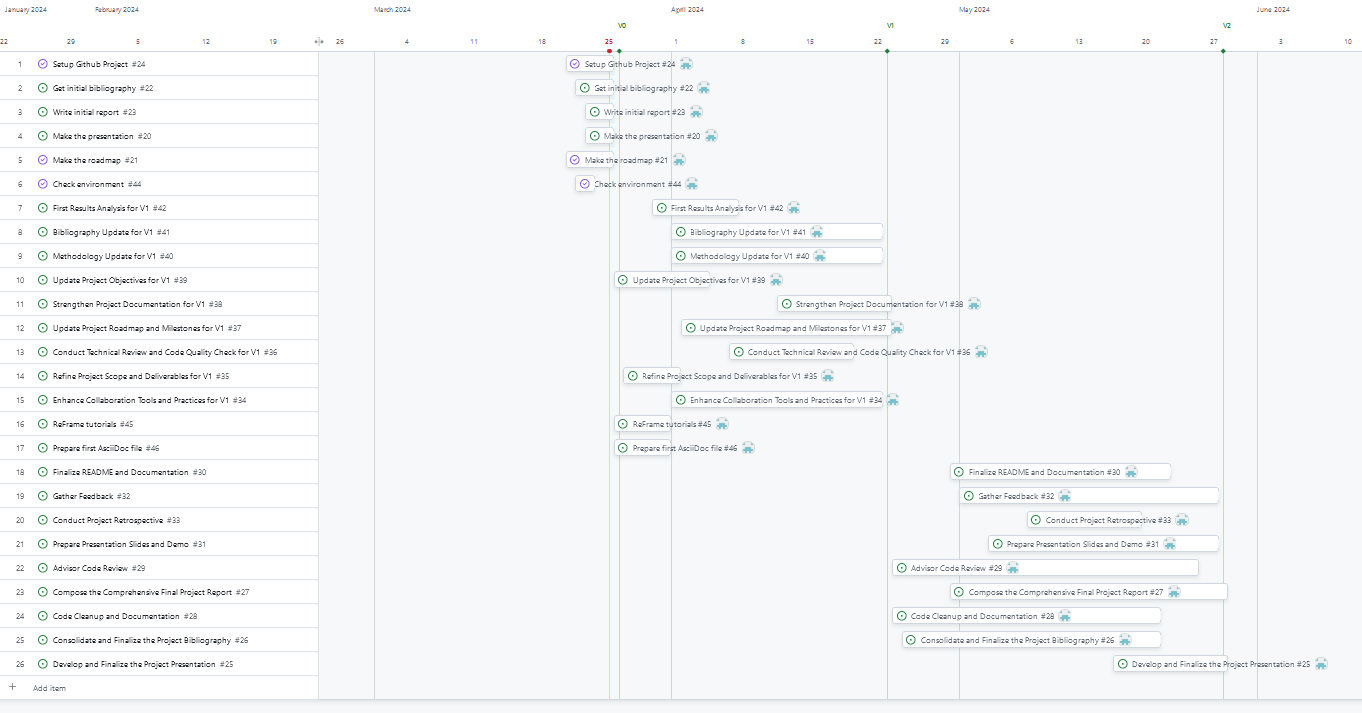
\includegraphics[width=\textwidth]{../../roadmap/roadmapv0-full.png}
    \caption{Roadmap v0}
    \label{fig:roadmapv0}
\end{figure}
\vspace{1cm}
At this moment, the roadmap has only been set up with generic project-conducting issues,
except from environment checking.\\
More precise project-relative points has to be defined and added for v1.

\newpage
\section{Bibliography}
\nocite{*}
\printbibliography[heading=none]

\end{document}